\chapter{Related Work}
The \acrfull{ecu} of the \acrshort{had} system are in charge of comprehending the environment and making the right decisions. To accomplish high-level tasks like course planning and collision avoidance, the \acrshort{had} system has to estimate a more detailed 3D bounding box within the real world. The fundamental part of the ECU that manages perception, judgment, route planning, etc. is the  \acrfull{dnn}. The quantity and quality of annotated training data are the primary determinants of DNN performance. The main issue that arises while training a DNN based on point clouds is the scarcity of ground truths, which severely restricts the network's ability to converge quickly and perform at its best. More data is required for DNN to reduce the problem of class imbalance, enhance generalization, and prevent overfitting of the model.

One interesting approach that makes it simple to collect all ground truth labels is synthetic data simulation. Utilizing computer graphics techniques, efforts have been made to produce artificially labeled data \parencite{SuQLG15, 8462926, abs-1809-08495}.  Using the video game engine's APIs from Grand Theft Auto V (GTA-V), \parencite{abs-1804-00103} gathers the calibrated pictures and point cloud and uses this information for vehicle recognition in subsequent projects \parencite{8462926}. Simulators like AutonoVi-Sim, \acrshort{carla}  \parencite{8575306, Dosovitskiy17} are also employed for purely synthetic data generation. The \acrlong{cg} world has a restricted scale and complexity and is primarily created by hand. Although it is demonstrated that using these simulated data might enhance DNN performance, there are still certain issues like domain gaps\parencite{zero_domain_gap, care_real_and_syn_gap} that need to be resolved. 

\section{Data Augmentation}
\acrfull{da} has been extensively investigated for 2D images \parencite{transfsim2000, NIPS2000_ba9a56ce} and has shown enormous possibilities in training effective \acrshort{dnn} models with restricted training images. \acrshort{da} tries to modify and create new training samples in order to extend the variety of the training data. \parencite{xiao2022polarmix} . \acrshort{da} is now a standard pre-processing step when training a neural network, as its efficacy has been demonstrated across a wide range of tasks (NEED TO INSERT CITATION). In \parencite{abs-1708-01566}, the real-world image dataset is enhanced by the addition of rendered automobiles, which benefits from the foreground's variance and the background's realism. For the 2D image domain, several data augmentation methods are covered. In Cutout \parencite{cutout}, sections of the image are taken off to enhance an image patch. MixUp \parencite{mixup} combines two images and the corresponding labels. CutMix \parencite{cutmix} is a technique that replaces a part of an image with a patch from another image, combining Cutout and MixUp. Though many efforts have been made on image augmentation, very few concentrate on point cloud data augmentation.

Various augmentation methods for enhancing 3D point clouds have been comprehensively examined in \parencite{DBLP:journals/corr/abs-2004-01643} such as Global Augmentation, Local Augmentation, GT-Filtering and GT-Sampling.
Global Augmentation techniques are deployed across the entirety of the point cloud representing a scene, while local augmentation techniques are specifically targeted toward points associated with individual objects within the scene. All points of the point clouds and all annotations are concurrently subjected to global augmentations. Global augmentation encompasses a variety of techniques, including global translation, rotation, scaling, random flipping, and ground removal. In contrast to global augmentation, local augmentation techniques also involve translation, rotation, and scaling. However, the key distinction lies in their application: rather than applying these transformations to every point indiscriminately, they are exclusively applied to individual annotations and the points contained within those annotations. This approach ensures that each annotation is augmented independently from others, with unique random values drawn for each annotation. The GT-Filtering method serves as a means to filter ground truth objects. This filtering process can be contingent upon various factors, such as difficulty level (difficulty level as described in KITTI \parencite{Geiger2012CVPR}) or the number of points contained within the objects. GT-Sampling involves the process of sampling additional ground truth objects, like individuals, from different scenes and integrating them into the current scene. To accomplish this, it's necessary to iterate through all annotations once and create a database that associates annotations with their respective points. This approach is employed to address the imbalance between "foreground" and "background" in datasets like SemanticKITTI \parencite{behley2019semantickitti}, thereby aiming for more balanced datasets. The subsequent section delves into various lidar augmentation strategies, exploring methods to enhance lidar data for improved performance in tasks such as object detection, segmentation, and classification.

\section{Augmentation Strategies involving LiDAR point cloud}

This section provides a detailed examination of different augmentation strategies concerning lidar point clouds. The emphasis is placed on elucidating the key features and characteristics of each strategy, delineating their significance in enhancing the quality and diversity of lidar data for various applications. 
\begin{itemize}
    \item \textbf{SECOND: Sparsely Embedded Convolution Detection} : In this study \parencite{second2018}, a database was constructed to store the labels of all ground truth objects and their corresponding point cloud data derived from the training dataset's 3D bounding boxes. During the training process, a subset of ground truth objects was randomly selected from this repository using GT-Sampling methodology and integrated into the current training point cloud through concatenation. This augmentation strategy aimed to augment the number of ground truth objects per point cloud, thus facilitating the simulation of objects existing in varied environmental conditions. Consequently, the detection performance was enhanced; however, it was noted that the approach did not account for the occlusion relationships between different augmented objects and between augmented objects and background points, thereby disregarding the importance of rational placement and occlusion considerations. Overall, the augmentation technique primarily relied on the simple reuse of ground truth objects.
    \item \textbf{Mix3D} : In this methodology \parencite{mix3d2021}, several augmentation techniques is employed to enhance the diversity and robustness of the lidar point cloud data. Firstly, the translation of multiple scenes to the origin was carried out by subtracting the centroid from all point positions, ensuring uniformity in spatial orientation. Subsequently, random transformations such as flipping in both horizontal directions and random rotations along different axes is applied to introduce variability. Additionally, random sub-sampling, elastic distortion, and random scaling is implemented, along with possible contrast augmentation, random brightness adjustments, and color jittering. Post-augmentation, the augmented point clouds from both scenes is merged by simply combining their points, effectively forming the union of the two sets. Furthermore, to augment the data out-of-context, points from two scenes is concatenated, serving as a valuable augmentation strategy, particularly useful for tasks like semantic segmentation.
    \item \textbf{LiDAR-Aug} : This research endeavor \parencite{lidar_aug}, introduces a rendering-based framework specifically designed to augment LiDAR point cloud data. By leveraging rendering techniques, augmented objects are seamlessly integrated into real background frames, ensuring the automatic enforcement of occlusion constraints. Furthermore, a novel method is proposed for incorporating CAD models into scenes and generating augmented LiDAR point clouds using a rendering module. The framework also utilizes the lightweight "ValidMap" method to generate poses for augmented objects, ensuring collision avoidance and achieving more realistic obstacle placements. Moreover, improvements are made over GT sampling by implementing measures to avoid object collisions during the object insertion process.
    \item \textbf{Augmented LiDAR Simulator for Autonomous Driving} : This study \parencite{aug_lidar_sim_2020} presents a lidar point cloud simulation framework  designed to enrich real point clouds by incorporating synthetic obstacles. The synthetic obstacles, represented by movable CAD models, encompass various types, with 500 models dedicated to pedestrians, 45 models allocated for cars, SUVs, etc. Real-world background models acquired using the RIEGL scan device, renowned for its high-speed, high-performance dual scanner mobile mapping system capabilities, are seamlessly integrated with semantic information. Background annotation using semantic segmentation information obtained through PointNet++ \parencite{pointnetplus2017} is employed, with annotations meticulously refined through filtration by groups of annotators. Additionally, the framework incorporates realistic obstacle placement learned from real traffic scenes to ensure the authenticity and accuracy of the augmented point cloud environment.
    \item \textbf{LiDARsim} : In this simulation-based approach \parencite{lidarsim2020}, the scan background is replaced with a method involving LiDAR data registration and fusion of multiple frames, while dynamic objects is reconstructed from point cloud data rather than relying on synthetic CAD models. To facilitate this, a substantial catalog comprising 3D static maps and dynamic objects is first compiled through extensive drives across different cities with the self-driving fleet. Scenarios is subsequently generated by selecting scenes from this catalog and virtually placing a self-driving vehicle (SDV) and dynamic objects within the chosen scenes, ensuring plausible and realistic arrangements.
    \item \textbf{PointMixup} : PointMixup \parencite{pointmixup2020} introduces an interpolation method inspired by MixUp \parencite{mixup} in image augmentation. This approach generates new examples by optimally assigning the path function between two labeled training point clouds.
    \item \textbf{PointAugment} : This augmentation method \parencite{pointaugment2020}is utilized for automatically optimizing and augmenting point cloud samples during the training of classification networks through the use of an augmentor to enhance data diversity. This method is employed to learn augmentation functions tailored to individual samples or classes, ensuring specificity in augmentation strategies. This approach integrates sample-aware auto-augmentation techniques and incorporates objectwise augmentor learning alongside classification learning using labeled training samples. However, the inclusion of an additional augmentor network and the intricate adversarial training process may introduce practical challenges to implementation.
    \item \textbf{PointPainting} : The proposed approach \parencite{pointpainting2019} involves initially executing an Image Segmentation network on the camera image. Subsequently, the predicted segmentation class scores are projected onto the LiDAR point cloud, effectively "painting" the point cloud with the segmentation results obtained from the camera image. This method offers an enhancement in 3D detection capabilities compared to the augmentation techniques.
    \item \textbf{PointAugmenting} : This research \parencite{pointaugmenting2021} introduces an object detection algorithm focusing on integrating 2D camera images with 3D LiDAR point clouds. In this methodology, deep features extracted by a 2D Object Detector from camera images are projected onto the corresponding points within the LiDAR point cloud. This process facilitates the fusion of information from the 2D image domain into the 3D LiDAR space, enhancing the feature representation and potentially improving object detection performance.
    \item \textbf{\acrfull{paaug}} : The proposed method \parencite{pa_aug2020} leverages the structural information of 3D ground-truth boxes to enable the network to learn intra-object relationships. It extends the GT-Sampling technique by partitioning GT objects into sub-partitions and introducing random augmentation to each partition, such as dropping all points within a partition. Objects such as cars, cyclists, and pedestrians from the KITTI dataset are utilized for this purpose. By dividing objects into multiple partitions and probabilistically applying lidar data augmentation operations like dropout, swapping, mixing, sparsifying, and introducing noise to each partition region, the method not only enhances the accuracy of the dataset but also demonstrates robust performance on corrupted data.
    \item \textbf{Augmentation of LiDAR for Fog Simulation} : A novel fog simulation method suitable for any LiDAR dataset is discussed in \parencite{fog_sim_2021}, focusing on achieving physically valid simulations. This method involves augmenting clear weather point cloud data with artificial fog, thereby enhancing the realism of the dataset. The strategy has enhanced the efficacy of 3D object detection under challenging atmospheric conditions characterized by the presence of fog.
    \item \textbf{Augmentation of LiDAR for Snowfall Simulation} :\parencite{snow_sim_2022} discusses augmenting the lidar point cloud to simulate real-world snowfall. Using this method, artificial snow is added to clear weather point clouds. With this method, each LiDAR line's snow particle sample is taken in two dimensions, and the resulting geometry is used to modify the measurement for each LiDAR beam.
    \item \textbf{Patch-based Progressive 3D Point Set Upsampling} \parencite{patched_up_2018} discusses the method of upsampling from lower resolution points to enhance resolution, aiming to reveal detailed geometric structures from sparse and noisy inputs.
    \item \textbf{\acrfull{sessd}} : In the proposed methodology \parencite{sessd_2021}, the ground truth bounding box is partitioned into six pyramid shapes by connecting the centroid with the faces of the box. Subsequently, random dropout, swap, and sparsify operations are applied to each subset of points derived from these divisions, effectively simulating partial object occlusion, increasing object diversity, and mimicking variations in point sparsity. This process treats the divided point subsets as disassembled parts, allowing for targeted manipulation. Prior to shape-aware data augmentation, a series of global transformations are applied to the input point cloud, including random translation, flipping, and scaling. Overall, this approach integrates both shape-aware and global transformations to augment the data effectively.
    \item \textbf{\acrfull{ppba}} : PPBA \parencite{ppba_2020} uses automated data enhancement methods to find the ideal settings for augmentation. During this procedure, the augmentation schedule is optimized by reducing the size of the search space and using the most effective parameters from previous rounds. It is discussed that sampling from individual frames of data from sensors results in a tenfold gain in data efficiency.
    \item \textbf{\acrfull{dada}} :  \parencite{dada_2023} In this approach, transformation of orthogonal coordinates of the point cloud into a spherical coordinate system is carried out, followed by sampling based on the lidar characteristics specific to the dataset, such as Velodyne HDL-64E for KITTI \parencite{Geiger2012CVPR} or a 40-beam lidar for the ONCE dataset \parencite{mao2021one}. The object is evenly sliced and sampled in accordance with the lidar resolution corresponding to the dataset's lidar characteristics. In the case of existing ground truth (GT) objects, points are simulated while adhering to the lidar characteristics to maintain the object's shape. Subsequently, downsampling or upsampling is performed based on the point density requirements.
    \item \textbf{PolarMix} : This method \parencite{xiao2022polarmix} presents an innovative way to mix in cylindrical coordinates at the object and scene levels. Swapping at the scene level involves slicing along the azimuth axis to exchange point cloud regions of two circular LiDAR scans. Mixing at the instance level involves copying the rotated point objects into additional scans after cropping them from one LiDAR scan and rotating them by various azimuth degrees to make several copies. It should be noted, nevertheless, that this approach does not take shadowing effects into consideration and can lead to the illogical positioning of instance objects.
    \item \textbf{PatchAugment} : The focus of this methodology \parencite{patch_aug_2021} is on enhancing data inside the immediate area or neighborhood of the sampled object, which principle is similar to the \acrshort{paaug} data augmentation technique.
    \item \textbf{PointCutMix} : Inspired by \acrfull{msda} in the image domain, this method \parencite{pointcutmix_2021} generates new training data by mixing the original training samples. Specifically, subsets of point objects are replaced with those of other objects to enrich the training data. To utilize this approach, annotated point cloud objects from two point clouds with corresponding labels are required.
    \item \textbf{RS-Aug} : This approach \parencite{rs_aug_2023} involves constructing an augmented reality scene to enhance the diversity of the training dataset. Initially, a pre-trained semantic segmentation model, RangeNet++ \parencite{rangenetplus2019}, is utilized to estimate semantic labels. This step serves as a preprocessing stage for the creation of a database in the auto-annotation process. Subsequently, the database is sampled for rendering augmentation in the subsequent step.
    \item \textbf{\acrfull{br}} : In this approach \parencite{xu2022reality}, position-level annotation is employed to build a virtual scene using an existing object database, facilitating weakly supervised 3D object detection. This process entails labeling the center of each object in the 3D space, followed by generating a virtual scene from a repository of 3D shapes.
    \item \textbf{Object Insertion Based Data Augmentation for Semantic Segmentation} : Using this method \parencite{9811816}, annotated LiDAR point clouds are used to extract foreground objects, which are then upsampled to create an object library. Objects are dynamically introduced into the LiDAR point cloud during training. Parameters similar to actual LiDAR settings are used to mimic realistic scanning lines and shadows by using range images, which are generated depending on the resolution of the LiDAR used for data gathering.
    \item \textbf{PointWOLF} : To enhance the variation of known 3D objects, this approach \parencite{pointwolf_2021} uses weighted alterations within local neighborhoods. It might be used, for example, on objects like wolves to produce different poses. The needed diversity is obtained by carefully combining several local transformations that are done with regard to anchor points in smoothly varied ways.
    \item \textbf{Real3D-Aug} : In this method \parencite{sebek2022real3daug}, objects are strategically placed at the same distance with identical observation angles to ensure consistent object point density and LiDAR intensity across the dataset. Additionally, collision avoidance measures are implemented by analyzing overlapping bounding boxes within semantic datasets.
    \item \textbf{Contextual Ground Truth Sampling} : In order to rectify data imbalances and insert ground truth \acrshort{gt} objects in realistic placements, this method \parencite{lee2022resolving} uses contextual GT sampling (sampling ground truth objects from a pre-saved GT database).
\end{itemize}

\section{Need of the Thesis work}

The majority of augmentation methods primarily aim to enhance model performance for detecting specific classes using pre-labeled class instances. Many existing strategies assume prior knowledge of ground truth objects, with some leveraging state-of-the-art semantic models to obtain this information \parencite{rs_aug_2023}. However, occlusions are often overlooked is some augmentation strategies \parencite{second2018, xiao2022polarmix}, and accurate 3D bounding boxes are typically required for appropriate object insertion into the scene. While some approaches utilize a database of rendered graphics models of objects \parencite{second2018, rs_aug_2023}, simulators often rely on CAD models, which may exhibit unrealistic appearances, necessitate costly manual construction, and lack scalability to represent the diversity and complexity of real-world scenarios. Additionally, certain augmentation methods require knowledge of the lidar configurations used for the target dataset to facilitate augmentation effectively \parencite{9811816, dada_2023}. 
Data-driven LiDAR semantic segmentation methods frequently exhibit a decrease in accuracy when applied to unseen LiDAR configurations, as elucidated in \parencite{10204248}. This discrepancy results in a performance decline in LiDAR semantic segmentation tasks when the LiDAR used for collecting the test set differs from the LiDAR utilized for the training set. The variance in sampling patterns across various LiDAR configurations, characterized by differences in vertical and horizontal resolution, contributes to the emergence of sensor bias issues in 3D perception algorithms \parencite{survery_domain_adp_2021, domain_adp_appr_2020}. 
Certain augmentation techniques, like PA-AUG and PointWolf, concentrate only on enhancing the ground truth (GT) objects, they do not handle how these objects are combined with the surrounding scene. 
Current augmentation strategies rely on either known labeled data or semantic models to extract ground truth objects. However, there could be situations where the label of the ground truth objects to be extracted is unknown. \acrshort{sota} semantic models may also prove ineffective, as the model may not have encountered the specific object during the training. This highlights the need for alternative approaches to handle scenarios where ground truth information is unavailable or difficult to obtain.

\begin{figure}[htbp]
    \centering
    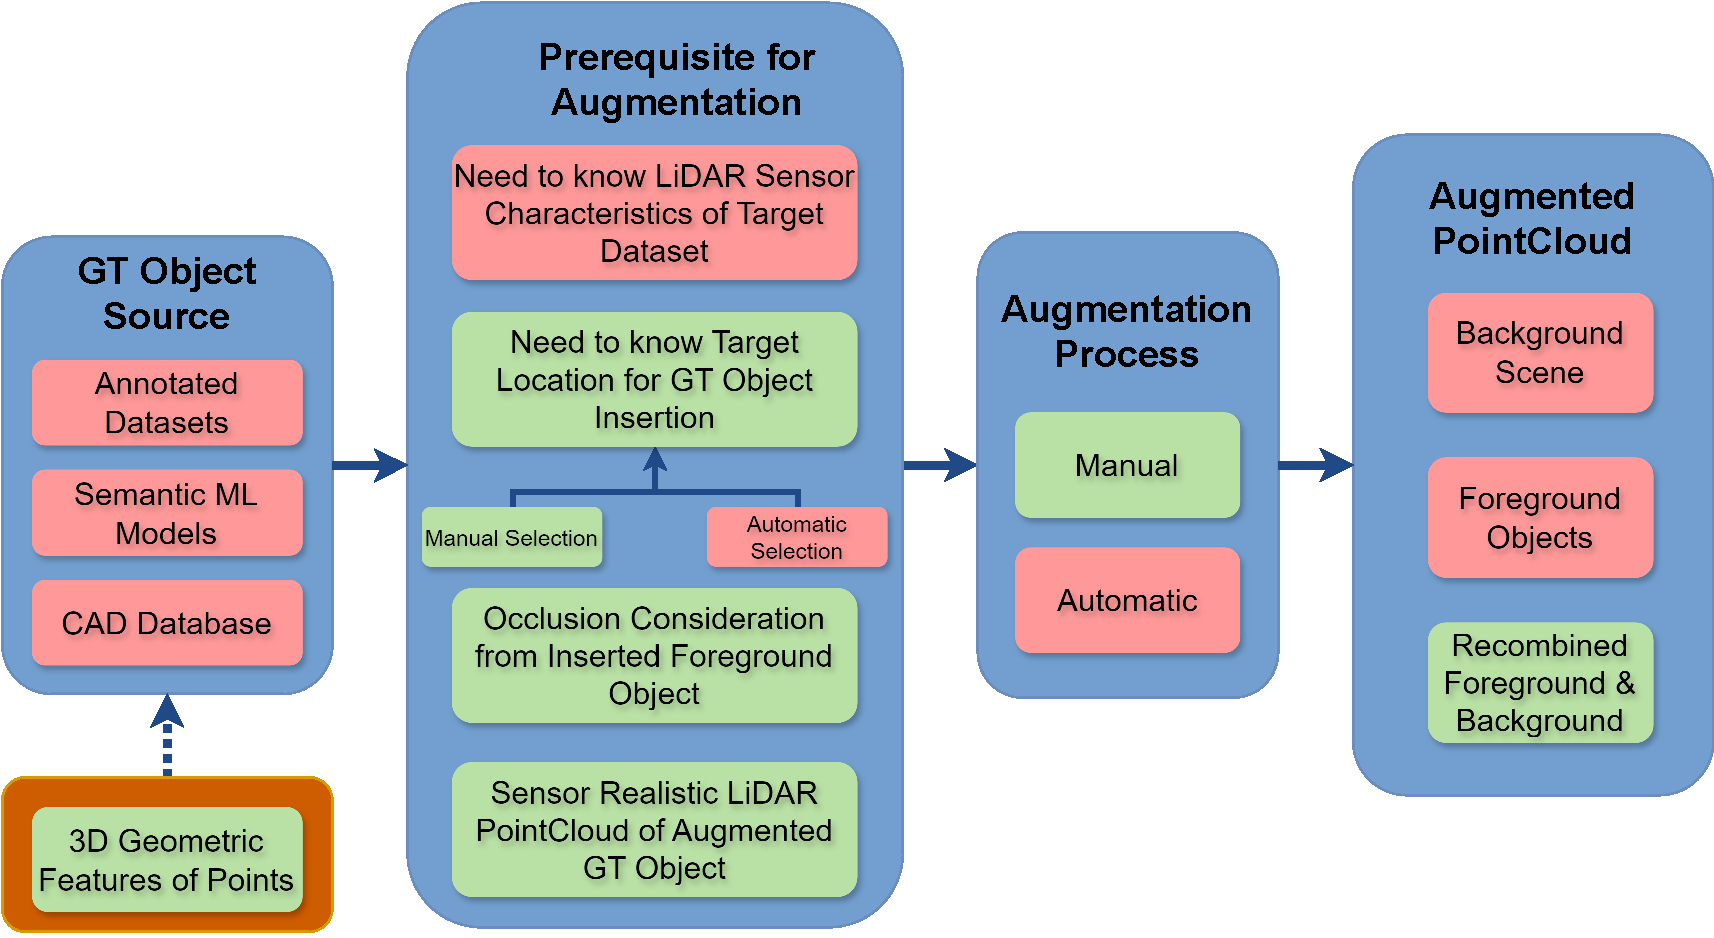
\includegraphics[width=1\linewidth]{97_graphics//related_work/related_work_block_diagram.pdf}
    \caption{Augmentation process of LiDAR Point Cloud}
    \label{fig:sota-related_work_block_diagram}
\end{figure}

In Figure \ref{fig:sota-related_work_block_diagram}, the blue-colored blocks denote the existing methods utilized for augmenting LiDAR point clouds. A unique aspect of this thesis is the utilization of 3D geometric features of points for ground truth object extraction within a scene, depicted by the dark orange-colored block. The green-colored blocks represent the methods utilized in the thesis for the generation of new scenarios.